\documentclass{article}

\usepackage{tikz}
\usetikzlibrary{calc}

% Smaller margins
\usepackage[
a4paper,
landscape,
left=2cm,
right=2cm,
top=2cm,
bottom=2cm,
footskip=1cm
]{geometry}

% Remove page numbers
\pagestyle{empty}

\begin{document}
\centering

\resizebox{1\textwidth}{!}{%
\begin{tikzpicture}
  \pgfmathsetmacro{\RectX}{1}
  \pgfmathsetmacro{\RectY}{1}
  \pgfmathsetmacro{\RectWidth}{64}
  \pgfmathsetmacro{\RectHeight}{1}

  \draw (\RectX,\RectY) rectangle ++(\RectWidth,\RectHeight);

  \pgfmathsetmacro{\RectWidthMinusOne}{\RectWidth-1}
  \foreach \i in {1,...,\RectWidthMinusOne} {
    \draw ($(\RectX+\i,\RectY)$) -- ++(0,\RectHeight);
  }

  \pgfmathsetmacro{\LabelStep}{8}
  \pgfmathsetmacro{\LabelCount}{(\RectWidth-1)/\LabelStep}
  \foreach \i in {0,...,\LabelCount} {
    \pgfmathparse{int(\i*\LabelStep)}
    \node at ($(\RectX+\pgfmathresult+0.5, \RectY+\RectHeight+0.5)$) {\pgfmathresult};
  }
\end{tikzpicture}
}%

\vspace{0.5\textheight}

\resizebox{1\textwidth}{!}{%
\begin{tikzpicture}
  \pgfmathsetmacro{\RectX}{1}
  \pgfmathsetmacro{\RectY}{1}
  \pgfmathsetmacro{\RectWidth}{64}
  \pgfmathsetmacro{\RectHeight}{1}

  \draw (\RectX,\RectY) rectangle ++(\RectWidth,\RectHeight);

  \pgfmathsetmacro{\RectWidthMinusOne}{\RectWidth-1}
  \foreach \i in {1,...,\RectWidthMinusOne} {
    \draw ($(\RectX+\i,\RectY)$) -- ++(0,\RectHeight);
  }

  \pgfmathsetmacro{\LabelStep}{8}
  \pgfmathsetmacro{\LabelCount}{(\RectWidth-1)/\LabelStep}
  \foreach \i in {0,...,\LabelCount} {
    \pgfmathparse{int(\i*\LabelStep)}
    \node at ($(\RectX+\pgfmathresult+0.5, \RectY+\RectHeight+0.5)$) {\pgfmathresult};
  }
\end{tikzpicture}
}%

\end{document}
